\chapter{序論}
配管は気体,液体,粉粒対などの流体を輸送や配線の保護などを目的とする管のことである.
配管は電気配線やケーブルを保護する電気配管や,生活に必要な水を家庭や学校などに輸送する水道管など様々な場面で使用されており,私達の生活において重要な役割を担っている.
そのため,配管を運用するにあたって常に耐久性と安全性を保ち続ける必要性がある. \\

\section{研究背景}
BIM とは,Building Information Modeling の略称で,コンピュータ上に建築物や土木構造物などの立体モデルを形成し,設計から維持管理までのプロセスをデジタル化する新しいワークフローの一環である.
このBIMモデリングはこれまでの3Dモデリングとは大きく異なる.従来の3次元モデリングでは平面図などの2次元上で作成した図面を元に別途3次元のモデルを作成していた.
そのため,図面と3次元モデルが連動しておらず,設計変更がある度に図面と3Dモデルの両方を修正する必要があり効率的ではなかった.
しかし,このBIM手法は一つのデータを修正すると全てのデータが連動し,関係する図面の該当箇所が自動修正され,従来の方法よりも高校率で作業を行うことが可能になる.\\
配管は建築物の中でも日常生活に欠かせない存在である.生活に必要な物資を運用したり電線やケーブルを保護するために使用されるなど幅広い面で活用されているため常に耐久性と安全性が求めらている.
その配管の図面を作成する際にはアイソメトリック(アイソメ)図と呼ばれる立体を斜めから見た視点で表示した等角図が用いられる.
アイソメ図の例を図\ref{fig:f1}に示す.
\begin{figure}[htbt]
	\centering
	 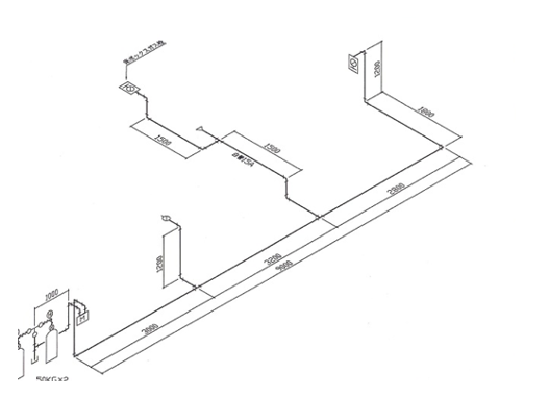
\includegraphics[height=75mm]{Figure/ex_iso.eps}
	 \caption{アイソメ図の例}
	 \label{fig:f1}
\end{figure}

このアイソメ図の最大の特徴は、図面を見るだけで配管のルートを直感的に理解しやすくなる点である。
設計図には平面図、立体図、系統図など、さまざまな種類があるが、配管の場合には配管同士が複雑に重なり合うことが多い。このため、左右上下からの視点では配管を見分けることが困難である。
一方、アイソメ図は配管のルートや交差する配管の前後関係を立体的に描画する手法として有効である.
従来のアイソメ図作成方法を図\ref{fig:f2}に示す。
\begin{figure}[htbt]
	\centering
	 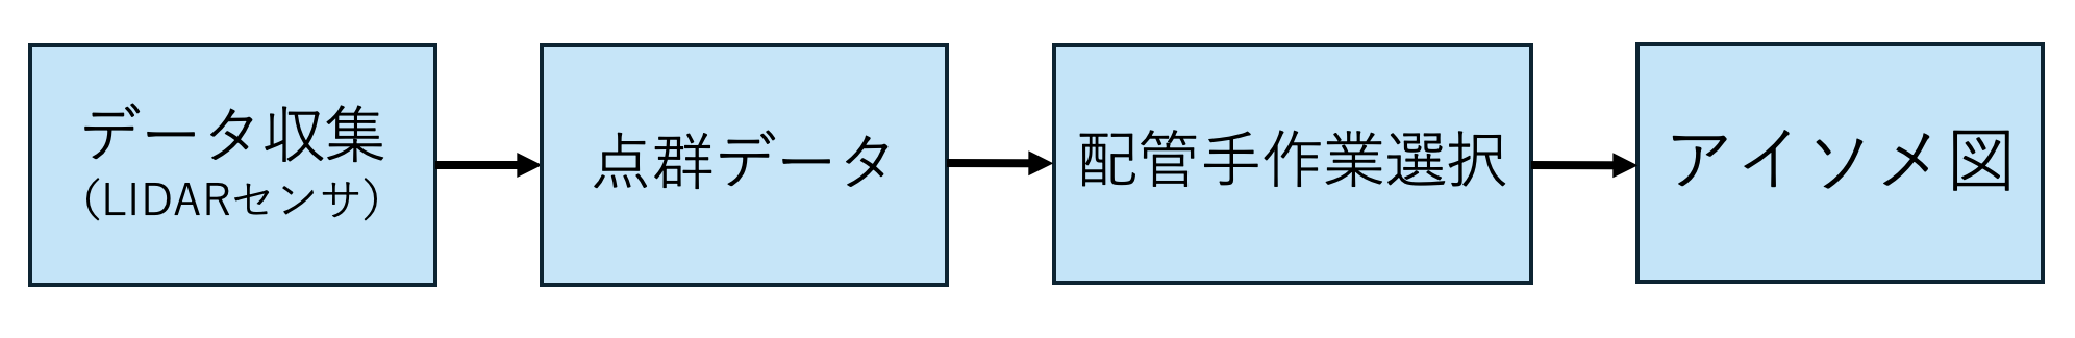
\includegraphics[height=22mm]{Figure/existing_research.eps}
	 \caption{従来のアイソメ図取得方法}
	 \label{fig:f2}
\end{figure}

アイソメ図の取得にはLight Detection and Ranging(LIDAR)と呼ばれる、レーザー光を用いて離れた物体の形状や距離を測定できるセンサを使用していた。
LIDARセンサは、距離情報を活用して三次元情報を取得できるだけでなく、広い測定範囲や高い精度を持つ点が評価されている。
しかし、その一方で、他のセンサと比較して高価であるというデメリットがあり、多くの人々が容易に利用できるものではなかった。

このような背景を受けて、近年ではLIDARセンサよりも安価なRGB-Dカメラを用いた認識手法が研究され始めている。
RGB-Dカメラとは、カラー画像と深度画像を同時に取得可能な、カラーカメラと深度センサが一体化したカメラである。
このカメラを用いることで、従来のLIDARセンサに比べて低コストでありながら三次元情報を取得することが可能となる。
図\ref{fig:f3}にRGB-Dカメラを用いて取得した配管画像の例を示す。
\begin{figure}[htbt]
	\centering
	 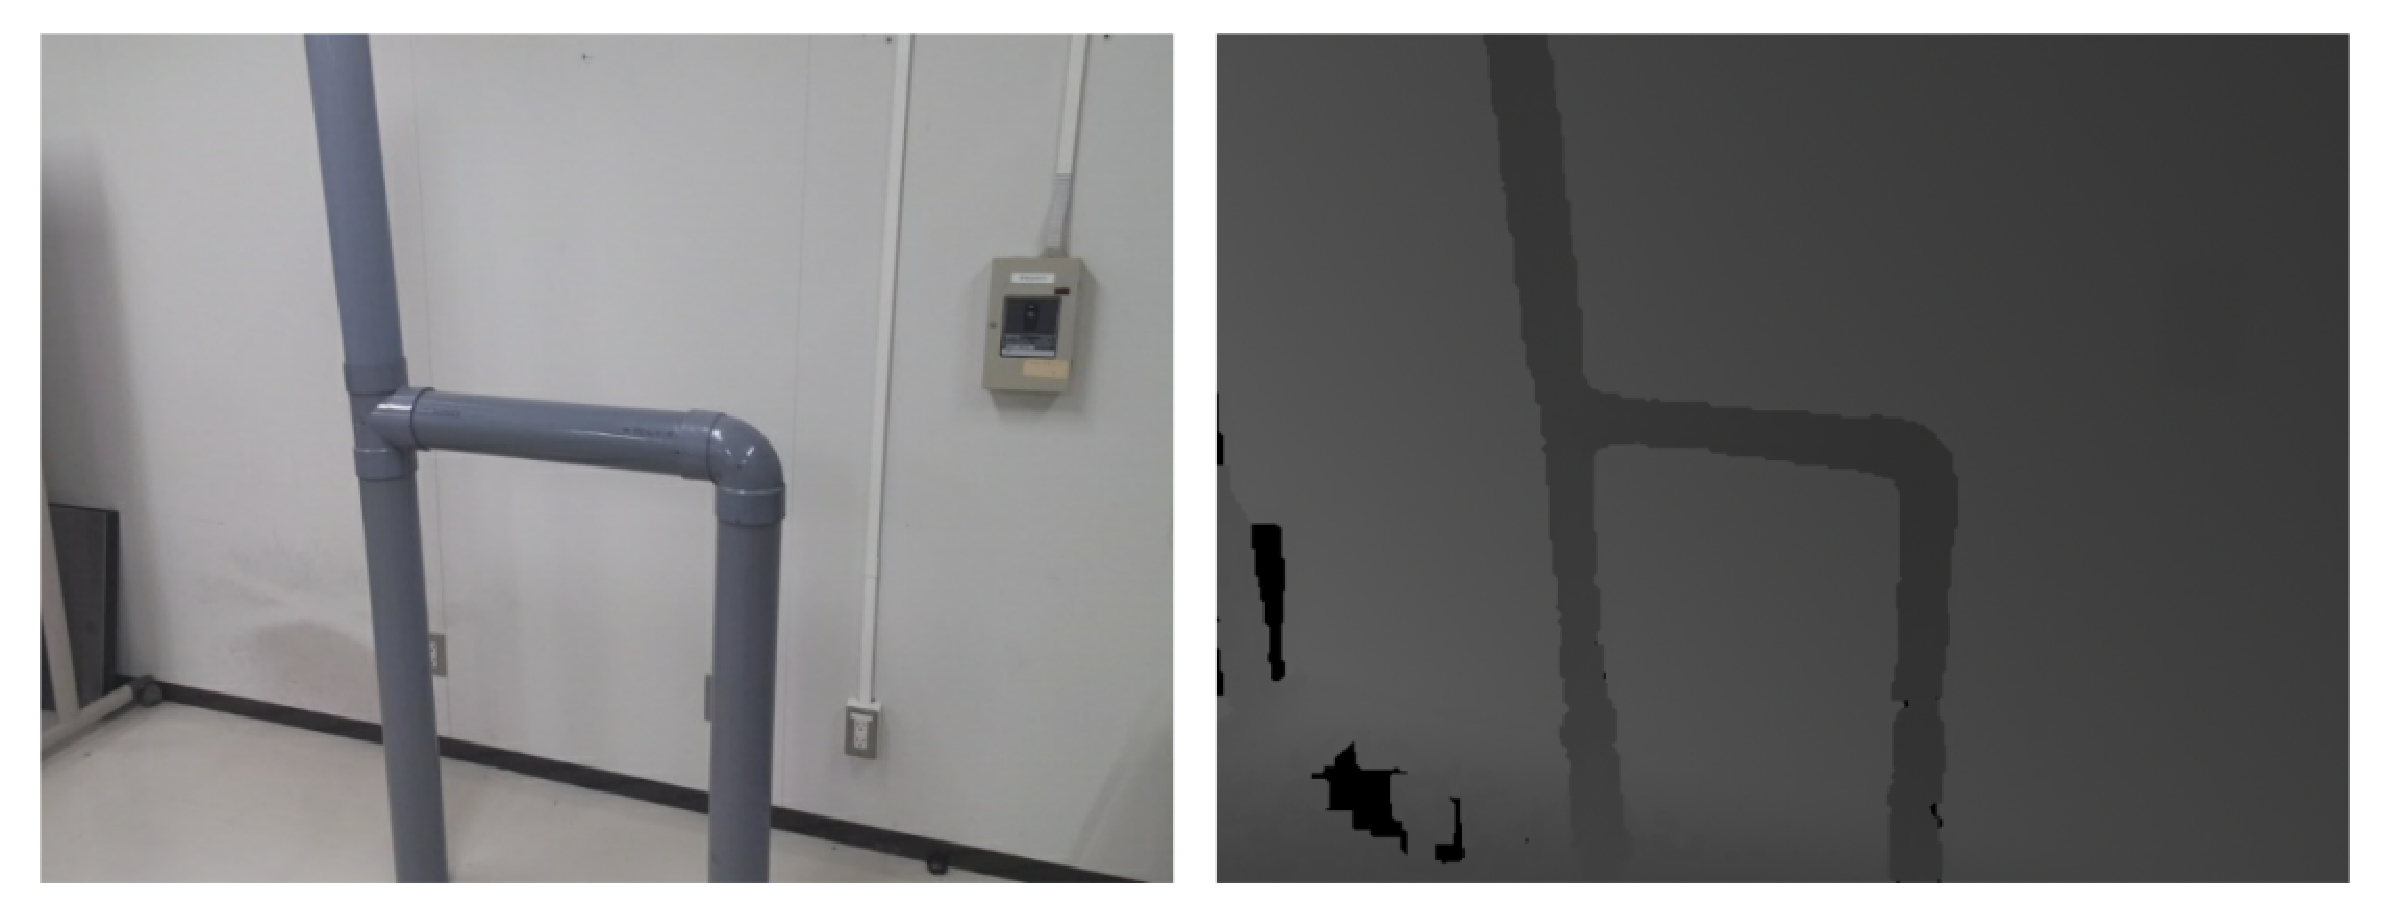
\includegraphics[height=55mm]{Figure/ex_pipe.eps}
	 \caption{RGB-Dカメラを用いて取得した配管画像の例}
	 \label{fig:f3}
\end{figure}

さらに、近年の画像認識分野では、機械学習を用いた研究が注目されている。
機械学習を導入することで業務効率化や生産性向上を実現できるだけでなく、人手不足の解消にも貢献できる。
そのため、今後も人工知能技術の利用は一層加速することが予測される。



\section{既存研究}
機械学習とは、コンピュータが膨大なデータを基にパターンを学習し、その規則性を抽出や活用する技術である。
その中でも、深層学習は人工知能の急速な発展を支える重要な技術の一つであり、人間の脳の構造を模倣したニューラルネットワークを用いた機械学習手法である。
従来の機械学習では特徴量を人間が設計する必要があったが、深層学習ではコンピュータがデータから自動的に特徴量を抽出し、より深い学習を通じて複雑な問題を解決できるようになった。
この技術は、画像認識や音声認識、データ分析など多岐にわたる分野で顕著な成果を上げている。

近年、深層学習を活用した画像認識技術の研究は急速に進展しており、物体検出、インスタンスセグメンテーション、さらに3次元位置姿勢推定といった主要なタスクで注目を集めている。
これらの技術的概要と代表的な手法を紹介する。

物体検出の代表的なモデルとして、YOLO(You Only Look Once)がある。

YOLOは、Convolutional Neural Network(CNN)を基盤としたニューラルネットワーク構造を使用し、画像中の物体を効率的に検出する(図\ref{fig:f4}参照)。
CNNとは、画像や映像データを解析する深層学習モデルであり、画像中のエッジや模様といった特徴を抽出し、それを基に分類や予測を行う技術である。
YOLOの特徴は、従来の物体検出手法が二段階に分けて行っていた境界設定と物体検出の処理を、一度に行う点にある。
この「End-to-End」の手法により、推定速度が大幅に向上し、リアルタイムでの物体検出が可能となった。


インスタンスセグメンテーションは、画像内の物体をピクセル単位で領域分割し、各領域に対応するクラスを識別する技術である。
物体検出が物体の位置を矩形で囲むだけであるのに対し、インスタンスセグメンテーションは物体の輪郭や形状を正確に捉えることができるため、物体の詳細な認識が可能となる。
インスタンスセグメンテーションの代表的なモデルとしてMask R-CNNがある。
\begin{figure}[htbt]
	\centering
	 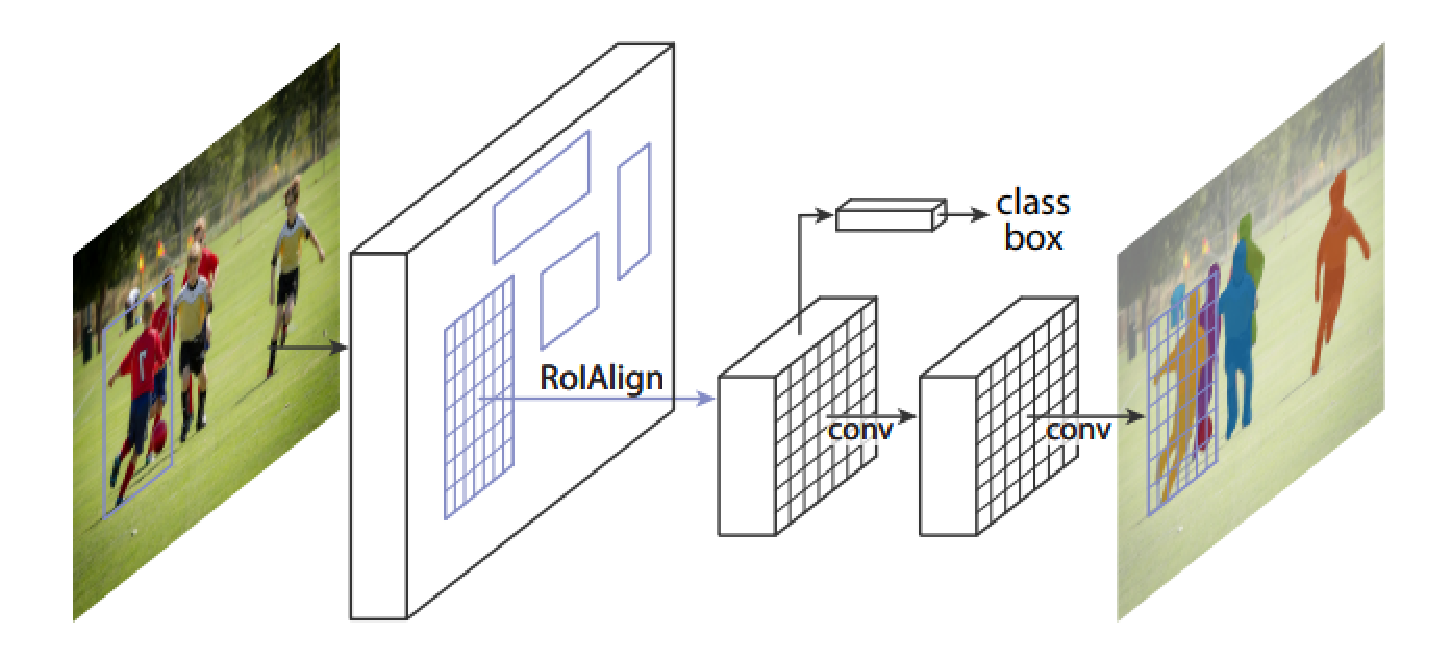
\includegraphics[height=55mm]{Figure/Mask-RCNN.eps}
	 \caption{インスタンスセグメンテーションMask RCNNのフレームワーク}
	 \label{fig:f5}
\end{figure}

Mask R-CNNは、物体検出において成功を収めたFaster R-CNNを基に、物体の位置を特定する領域提案ネットワーク(Region Proposal Network, RPN)と、物体の輪郭をピクセル単位で予測するマスク予測ネットワークを組み合わせた構造を持つ。
具体的には、RPNが画像内で物体が存在する可能性のある領域を提案し、その後、提案された領域に対してマスク予測ネットワークが物体の輪郭を正確に予測する。
このプロセスにより、物体の形状を詳細に認識することができ、従来の物体検出手法では対応できなかった、より複雑で精緻な解析が可能となる。

次に、3次元位置姿勢推定について紹介する。
3次元位置姿勢推定は、物体の位置(X, Y, Z)に加えて、回転や向き(Roll, Pitch, Yaw)を推定する技術であり、6自由度の姿勢を推定可能である。
ここでは、この技術を「6D姿勢推定」と呼ぶことにする。
6D姿勢推定を活用することで、配管の向きを特定し、それぞれの配管がどのように接続されているのかを把握することが可能となるため、アイソメ図作成において重要な役割を果たす。
6D姿勢推定の手法としては、RGB画像のみを入力として使用する方法や、Depth画像を併用する方法が存在する。

RGB画像のみを用いた代表的な手法の一つが、Gen6D(Generalizable Model-Free 6-DoF Object Pose Estimation from RGB Images)である。


この手法は、3Dデータを使用せず、カラー画像のみで物体の6D姿勢を推定できることを特徴としている。
従来、物体の姿勢推定には、認識対象物の3Dモデルを事前に作成し、それをデータセットに組み込む必要があったため、手間がかかっていた。
しかし、Gen6Dでは、3Dモデルを使用せず、カラー画像だけで高精度な姿勢推定を実現する。

Gen6Dの学習には、Colmapというソフトウェアを活用する。
Colmapは、Structure from Motion(SfM)技術を用いて、異なる視点から撮影された2D画像を基に3D点群を再構築し、その点群データを使用して物体の6D姿勢を推定する。

Gen6Dは、物体の姿勢推定を行うために、Detector(物体検出)、Selector(画像マッチング)、Refiner(姿勢補正)という3つのステップを経る。
まず、物体検出では参照画像をもとに物体の領域を検出し、次に画像マッチングでは、得られた領域画像と最も近い視点を持つ参照画像を選択する。
この参照画像の視点を用いて、物体の初期姿勢が推定される。
初期姿勢には誤差が生じることもあるが、画像マッチングはその誤差を最小化することを目指す。
最後の姿勢補正では、選ばれた参照画像からさらに6枚の画像を選び、これらの平均と分散を計算して初期姿勢を改良し、最終的な姿勢推定を行う。

ただし、Gen6Dにはいくつかの課題がある。
特に、学習には事前にSfMで点群データを準備する必要があり、この準備作業には時間と労力がかかる。
また、物体が重なり合うオクルージョンのような状況では、正確な姿勢推定が困難になるという課題がある。

一方、RGB-D画像を使用した手法としては、SAM-6D(Segment Anything Model for 6D Pose Estimation)が挙げられる。
\begin{figure}[htbt]
	\centering
	 \includegraphics[height=80mm]{Figure/SAM-6D.eps}
	 \caption{SAM-6Dの姿勢推定方法の流れ}
	 \label{fig:f7}
\end{figure}

図\ref{fig:f7}にSAM-6Dの姿勢推定方法の流れを示した。
Segment Anythingは、オブジェクトをゼロショットでセグメント化できるモデルであり、幅広い提案を生成する技術である。
Object Matchingは、この提案とターゲットオブジェクトの一致度を、セマンティクスや外見、形状を基に評価して有効なものを特定する。
Coarse Point Matchingは粗い対応でオブジェクトの初期姿勢を推定し、Fine Point Matchingはさらに詳細な対応を学習して正確な姿勢を求める方法である。
これらのプロセスが連携して、正確なセグメンテーションと姿勢推定を実現する。

また、オクルージョン(遮蔽)による影響を軽減するために、バックグラウンドトークンという仮想点を導入し、欠損領域があっても精度を維持する。
このアプローチにより、Gen6Dで課題となっていたオクルージョンに対処することが可能となる。


\section{研究目的}
本研究では、比較的安価で手軽に利用可能なRGB-Dカメラを活用し、計算効率に優れた深層学習ベースの手法を提案することで、一般的に利用可能なアイソメ図生成方法の確立を目指す。
図\ref{fig:f8}に新規のアイソメ図取得方法を示す。\\
\begin{figure}[htbt]
	\centering
	 \includegraphics[height=33mm]{Figure/new_research.eps}
	 \caption{新規のアイソメ図取得方法}
	 \label{fig:f8}
\end{figure}

従来のLIDARセンサの代替としてRGB-Dカメラを使用することで、低コストでアイソメ図を取得することが望める。
また、これまで配管検出処理は人間が手作業で行っていたが、本研究では深層学習を活用することで、検出処理の自動化と高効率化を実現する。

本研究の主な貢献は以下の通りである。
1つ目は、RGB-Dカメラを利用した低コストで汎用性の高いアイソメ図作成方法を提案し、広く使用可能なアプリケーションを提示したことである。
2つ目は、大規模配管設備のアイソメ図生成を実現するために、仮想環境で配管を構築し、実環境との差異を最小限に抑えた状態でアイソメ図を生成できるようにした点である。
3つ目は、アイソメ図作成に必要な6D姿勢推定モデルを比較検証し、本研究に適したモデルを選定したことである。


\section{本論文の構成}
本論文の構成は以下のようになる.
第1章では研究背景、既存研究、研究目的について述べる。
研究背景では、Building Information Modeling (BIM) の概要や、従来のアイソメ図取得方法について詳述する。
既存研究では、深層学習を用いた画像認識分野に関する研究を紹介し、これまでの手法との違いを明確にする。
研究目的では、本研究で提案する新たな手法とその貢献について述べる。

第2章では、深層学習を用いた配管6D姿勢推定およびアイソメ図作成に至る方法とその流れについて説明する。
第2.1節では本章の全体構成を紹介し、全体的な流れを把握できるようにする。
第2.2節では、RGB-D画像に基づく配管6D姿勢推定の方法について述べ、実際に使用する物体検出やセグメンテーション、6D姿勢推定モデルについて説明する。
第2.3節では、得られた6D姿勢推定情報を基にアイソメ図を作成する手法について述べる。
具体的には、配管の接続関係を推論し、アイソメ図を作成するためにCADデータに変換する方法を説明する。

第3章では、実環境における配管設備を用いた検証実験を通じて、提案手法の有効性を検証する。
第3.1節では使用する機材について説明し、必要な技術的要素を紹介する。
第3.2節では、データセットの収集方法およびデータセットの作成方法について説明する。
第3.3節では、提案手法の評価指標について述べ、実験結果の比較基準を明確にする。
第3.4節では、提案手法の有効性を確認するために行った実験結果について報告する。

第4章では、仮想環境における大規模配管設備での検証実験の結果を示す。
第4.1節では仮想環境の構築方法について説明し、仮想環境と実環境との差異を最小化するために導入したセンサーモデルについても詳述する。
第4.2節では、仮想環境で取得した配管画像を用いてアイソメ図を生成した結果を示し、その精度や効率について議論する。

第5章は結論にあたり、本研究の成果を総括し、今後の課題と展望について述べる。
